% Author: Till Tantau
% Source: The PGF/TikZ manual
\documentclass{minimal}

\usepackage{pgf}
\usepackage{tikz}
\usepackage[utf8]{inputenc}
\usetikzlibrary{arrows,automata}
\usetikzlibrary{positioning}


\tikzset{
    state/.style={
           rectangle,
           rounded corners,
           draw=black, very thick,
           minimum height=2em,
           inner sep=2pt,
           text centered,
           },
}

\begin{document}
% GENERAL GRAPH
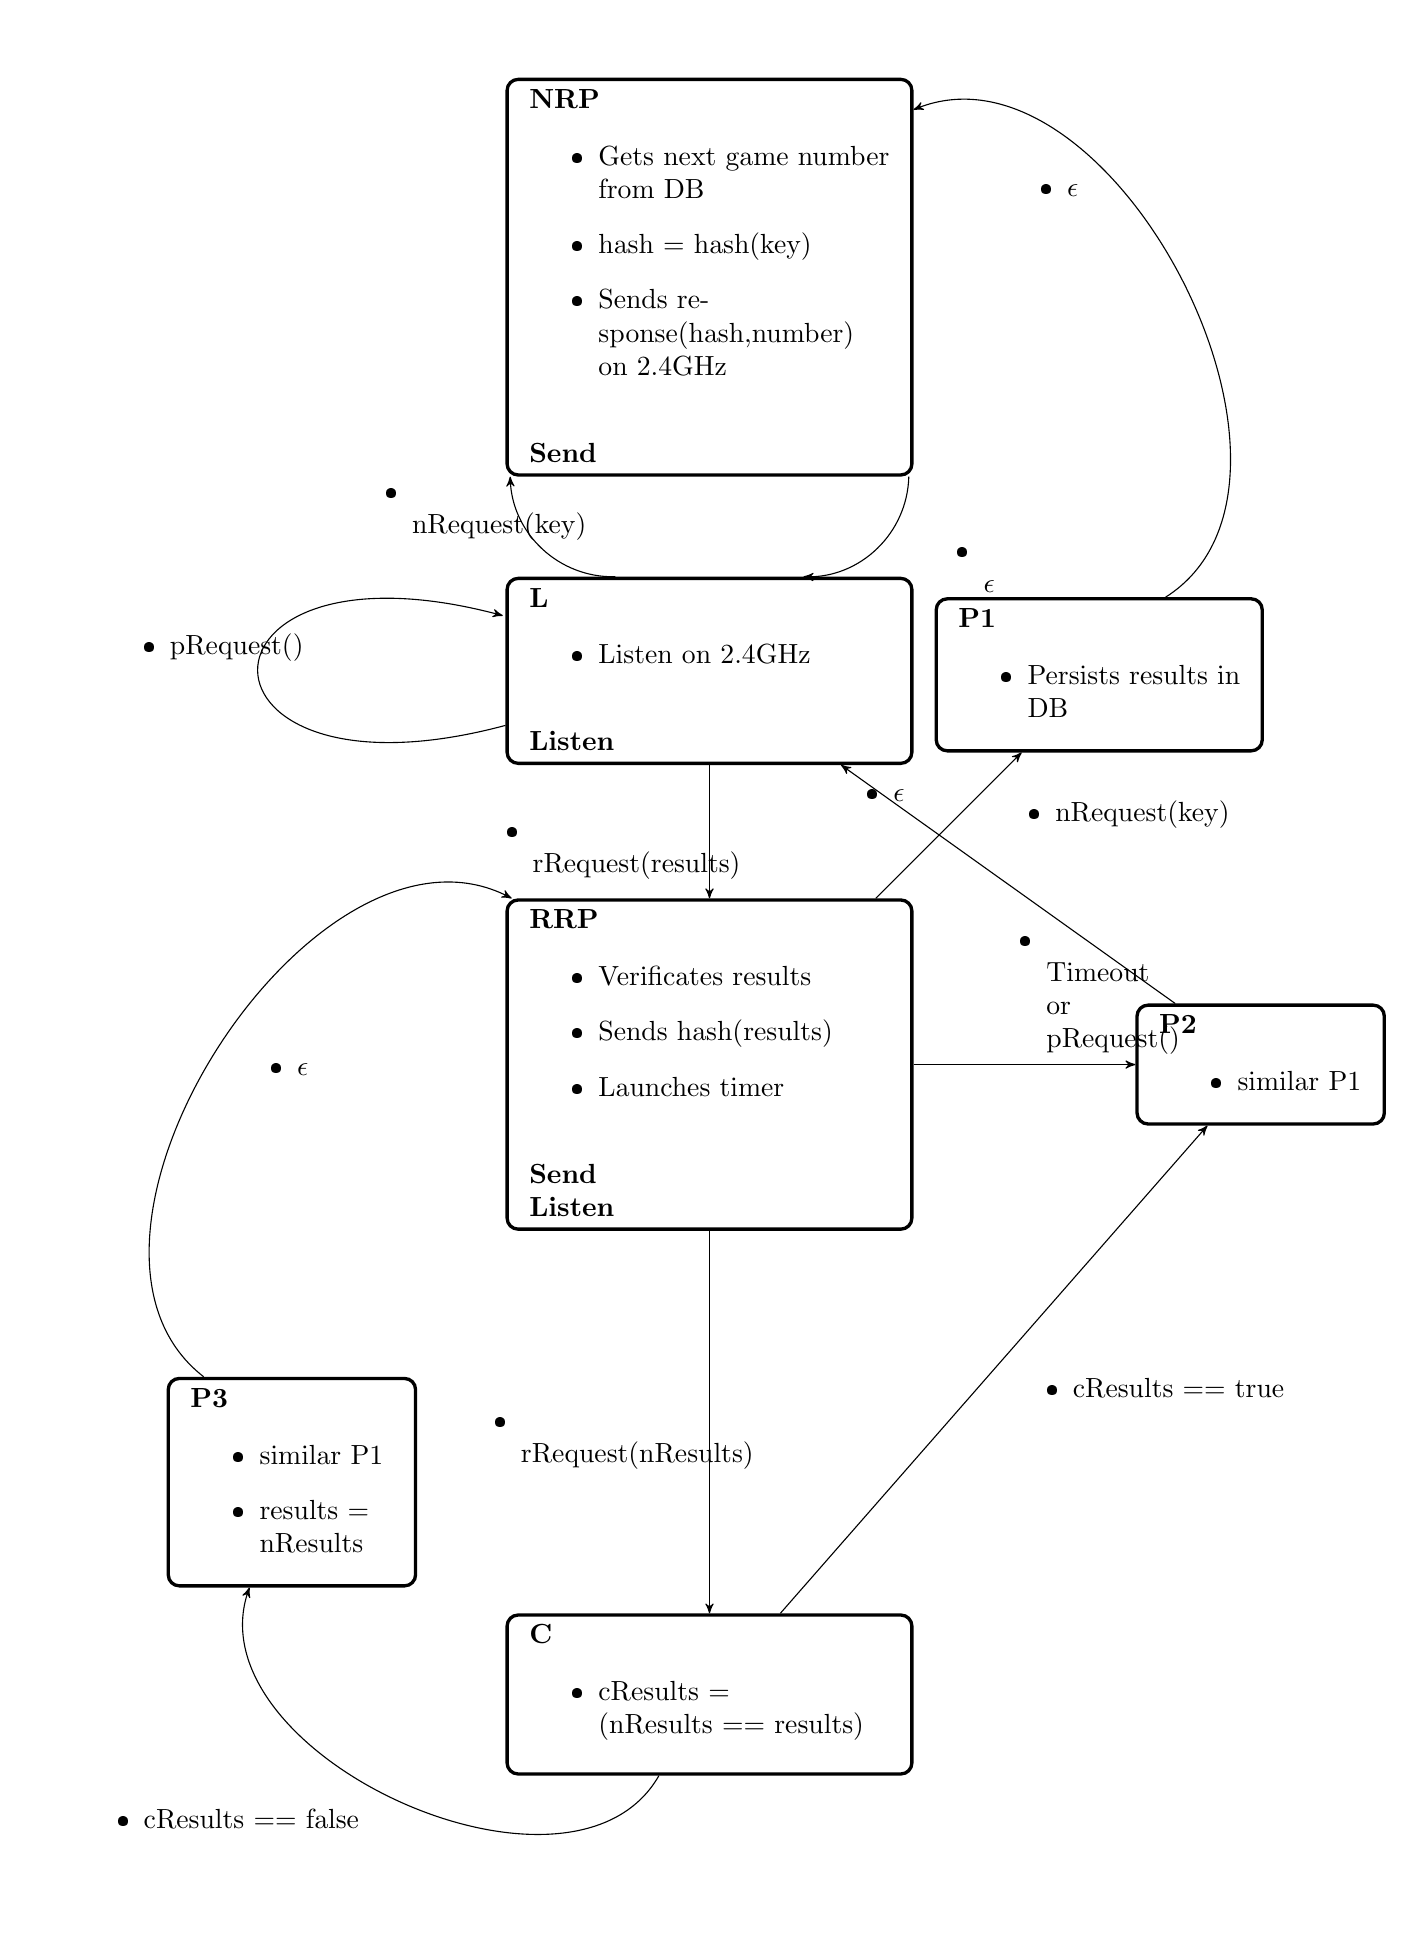
\begin{tikzpicture}[->,>=stealth']
   \node[state,
 node distance=5cm,
 text width=5cm] (L) 
 {%
 \begin{tabular}{l}
  \textbf{L}\\
  \parbox{5cm}{
  \begin{itemize}
   \item Listen on 2.4GHz
  \end{itemize}}\\ \\
  \parbox{3cm}{\mbox{\textbf{Listen}}}
 \end{tabular}
 };
  \node[state,
 above of=L,
 node distance=5cm,
 text width=5cm] (NRP) 
 {%
 \begin{tabular}{l}
  \textbf{NRP}\\
  \parbox{5cm}{
  \begin{itemize}
   \item Gets next game number from DB
   \item hash = hash(key)
   \item Sends response(hash,number) on 2.4GHz
  \end{itemize}}\\ \\
  \parbox{3cm}{\mbox{\textbf{Send}}}
 \end{tabular}
 };
  \node[state,
 below of=L,
 node distance=5cm,
 text width=5cm] (RRP) 
 {%
 \begin{tabular}{l}
  \textbf{RRP}\\
   \parbox{5cm}{
  \begin{itemize}
   \item Verificates results
   \item Sends hash(results)
   \item Launches timer
  \end{itemize}}\\ \\
  \parbox{3cm}{\mbox{\textbf{Send}}}\\
  \parbox{3cm}{\mbox{\textbf{Listen}}}
 \end{tabular}
 };

  \node[state,
 above right of=RRP,
 node distance=7cm,
 text width=4cm] (P1) 
 {%
 \begin{tabular}{l}
  \textbf{P1}\\
   \parbox{4cm}{
  \begin{itemize}
   \item Persists results in DB
  \end{itemize}}
 \end{tabular}
 };

  \node[state,
 right of=RRP,
 node distance=7cm,
 text width=3cm] (P2) 
 {%
 \begin{tabular}{l}
  \textbf{P2}\\
  \ \parbox{3cm}{
  \begin{itemize}
   \item similar P1
  \end{itemize}}
 \end{tabular}
 };
  \node[state,
 below left of=RRP,
 node distance=7.5cm,
 text width=3cm] (P3) 
 {%
 \begin{tabular}{l}
  \textbf{P3}\\
   \parbox{3cm}{
  \begin{itemize}
   \item similar P1
   \item results = nResults
  \end{itemize}}
 \end{tabular}
 };
  \node[state,
 below of=RRP,
 node distance=8cm,
 text width=5cm] (C) 
 {%
 \begin{tabular}{l}
  \textbf{C}\\
   \parbox{5cm}{
  \begin{itemize}
   \item cResults = \\(nResults == results)
  \end{itemize}}
 \end{tabular}
 };
 % draw the paths and and print some Text below/above the graph
\path 
  (L) edge[bend left=45] 
    node[anchor=south,left,text width=1cm,xshift=-4em,yshift=2em]
    {
      \begin{itemize}
        \item nRequest(key)
      \end{itemize}
    } 
    (NRP)
  (NRP) edge[bend left=45] 
    node[anchor=south,right,text width=1cm,xshift=1em]
    {
      \begin{itemize}
        \item $\epsilon$
      \end{itemize}
    } 
    (L)
  (L) edge  
    node[anchor=south,left,text width=3cm]
    {
      \begin{itemize}
        \item rRequest(results)
      \end{itemize}
    } 
    (RRP)
  (L) edge[loop left] 
    node[anchor=south,above,text width=4cm]
    {
      \begin{itemize}
        \item pRequest()
      \end{itemize}
    } 
    (L)
  (RRP) edge  
    node[anchor=south,right,text width=5cm,xshift=1em,yshift=1em]
    {
      \begin{itemize}
        \item nRequest(key)
      \end{itemize}
    } 
    (P1)
  (RRP) edge
    node[anchor=south,above,text width=1.2cm]
    {
      \begin{itemize}
        \item Timeout\\or\\pRequest()
      \end{itemize}
    }                    
    (P2)
  (RRP)  edge
    node[anchor=east,left,text width=3.5cm,xshift=1em]
    {
      \begin{itemize}
        \item rRequest(nResults)
      \end{itemize}
    } 
    (C)
  (C)  edge
    node[anchor=north,right,text width=4cm]
    {
      \begin{itemize}
        \item cResults == true
      \end{itemize}
    } 
    (P2)
  (C)  edge[bend left=85] 
    node[anchor=west,left,text width=4cm]
    {
      \begin{itemize}
        \item cResults == false
      \end{itemize}
    } 
    (P3)
  (P3)  edge[bend left=85] 
    node[anchor=west,right,text width=4cm]
    {
      \begin{itemize}
        \item $\epsilon$
      \end{itemize}
    } 
    (RRP)
  (P2)  edge 
    node[anchor=west,right,text width=4cm,yshift=4em,xshift=-7em]
    {
      \begin{itemize}
        \item $\epsilon$
      \end{itemize}
    } 
    (L)
  (P1)  edge[bend right=85] 
    node[anchor=west,right,text width=4cm,yshift=4em,xshift=-7em]
    {
      \begin{itemize}
        \item $\epsilon$
      \end{itemize}
    } 
    (NRP)
 ;
\end{tikzpicture}
\end{document}